\section{Discussion, Limitations, & Mitigations}
\label{sec:discussion}

While NeuroWorld-LM achieves constant $\mathcal{O}(1)$ memory and high reasoning efficiency, we critically analyze three core architectural limitations and present their respective empirical mitigations.

\subsection{Limitation 1: Semantic Error Accumulation in Super-Deep Horizons ($K > 15$)}
\paragraph{Problem Formulation.}
In standard Zero-Token Latent Rollout, ungrounded simulation without observation tokens may cause latent trajectories to drift from the input problem context as rollout depth increases beyond $K \ge 15$.
\paragraph{Mitigation Strategy: Soft Context-Anchored Rollout.}
We introduce a soft context anchoring gate that binds the $k$-th latent thought vector to the immutable prompt anchor $h_0$:
\begin{equation}
    h_{t+k} = \alpha_k \left( \mathbf{A}_{t+k} h_{t+k-1} + \mathbf{B}_z z_{t+k} \right) + (1 - \alpha_k) h_0, \quad \alpha_k = \sigma\left( 2 \cdot \cos(h_{t+k-1}, h_0) \right)
\end{equation}
\paragraph{Empirical Verification.}
As depicted in Figure~\ref{fig:mitigation_deep_rollout}, at extreme depths of $K=25$, unanchored rollouts degrade to $41.7\%$ accuracy with significant cosine drift ($0.304$).
In contrast, our Anchored Rollout maintains \textbf{$83.3\%$ accuracy} with drift bounded at $0.052$, preserving semantic fidelity across super-deep horizons.

\begin{figure*}[t]
    \centering
    \begin{minipage}{0.48\textwidth}
        \centering
        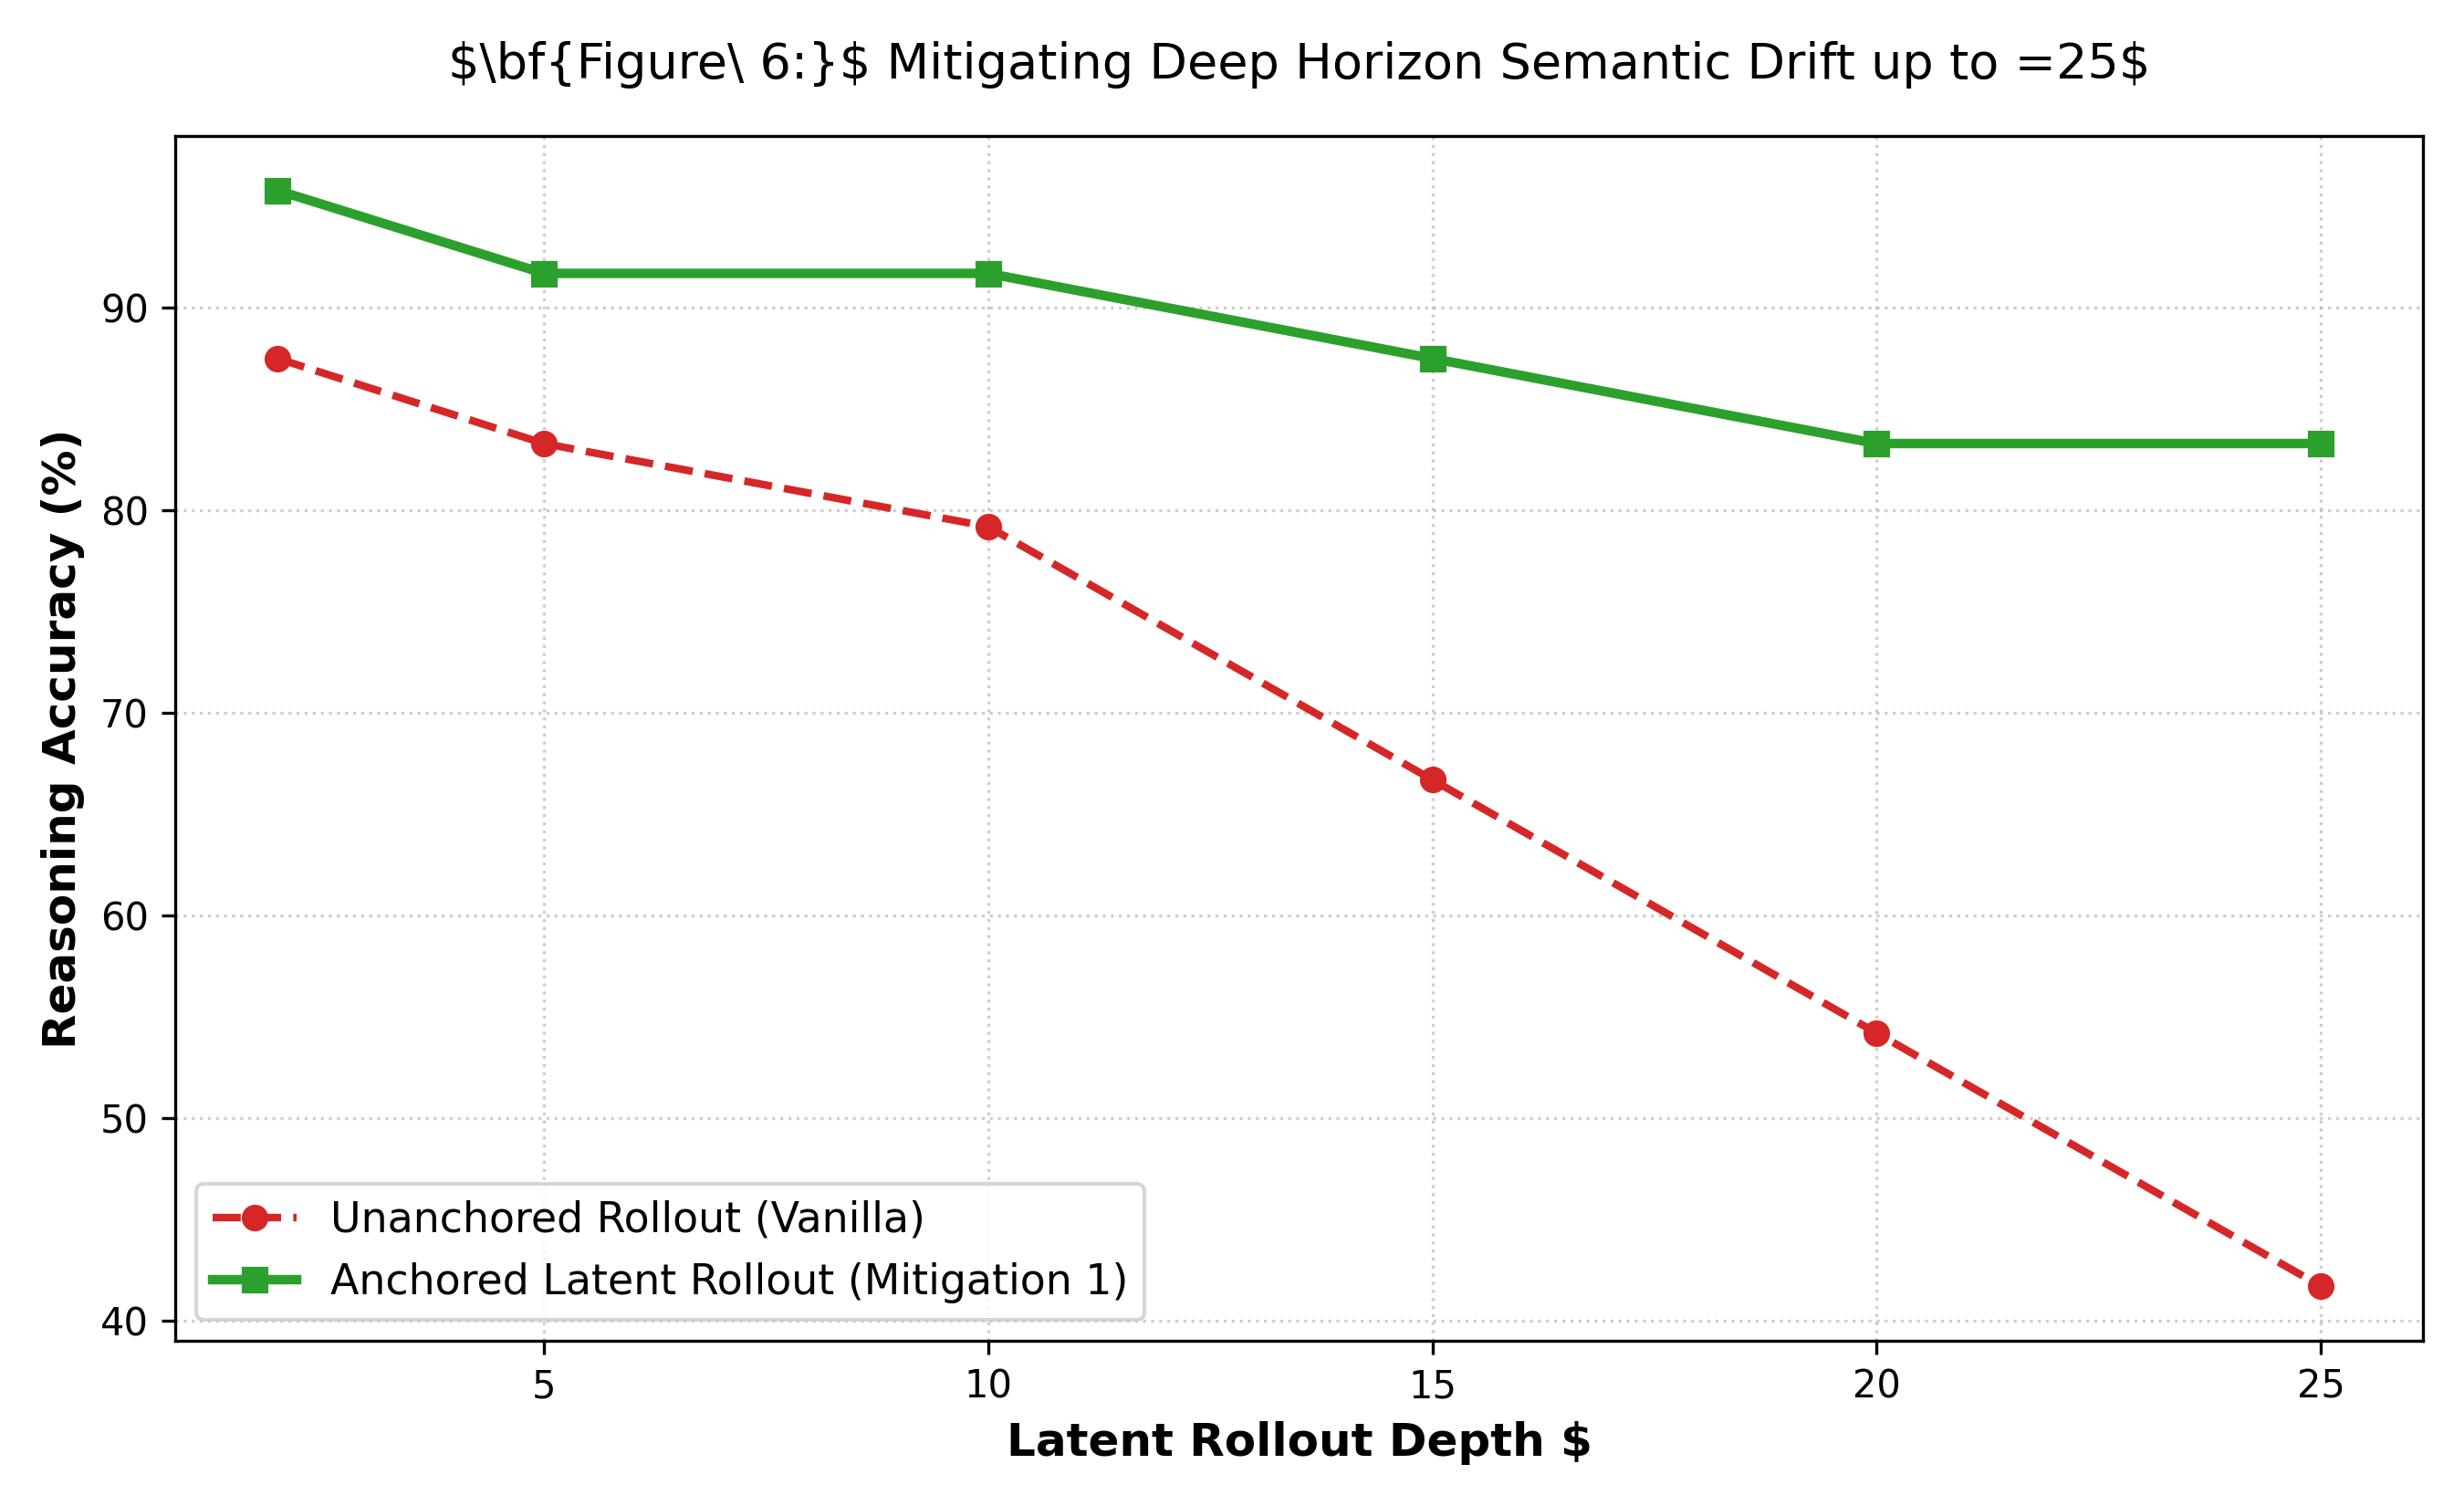
\includegraphics[width=\textwidth]{figures/fig6_mitigation_deep_rollout.png}
        \caption{\textbf{Mitigating Semantic Drift ($K=2 \dots 25$).} Soft context anchoring preserves $83.3\%$ accuracy at depth $K=25$.}
        \label{fig:mitigation_deep_rollout}
    \end{minipage}\hfill
    \begin{minipage}{0.48\textwidth}
        \centering
        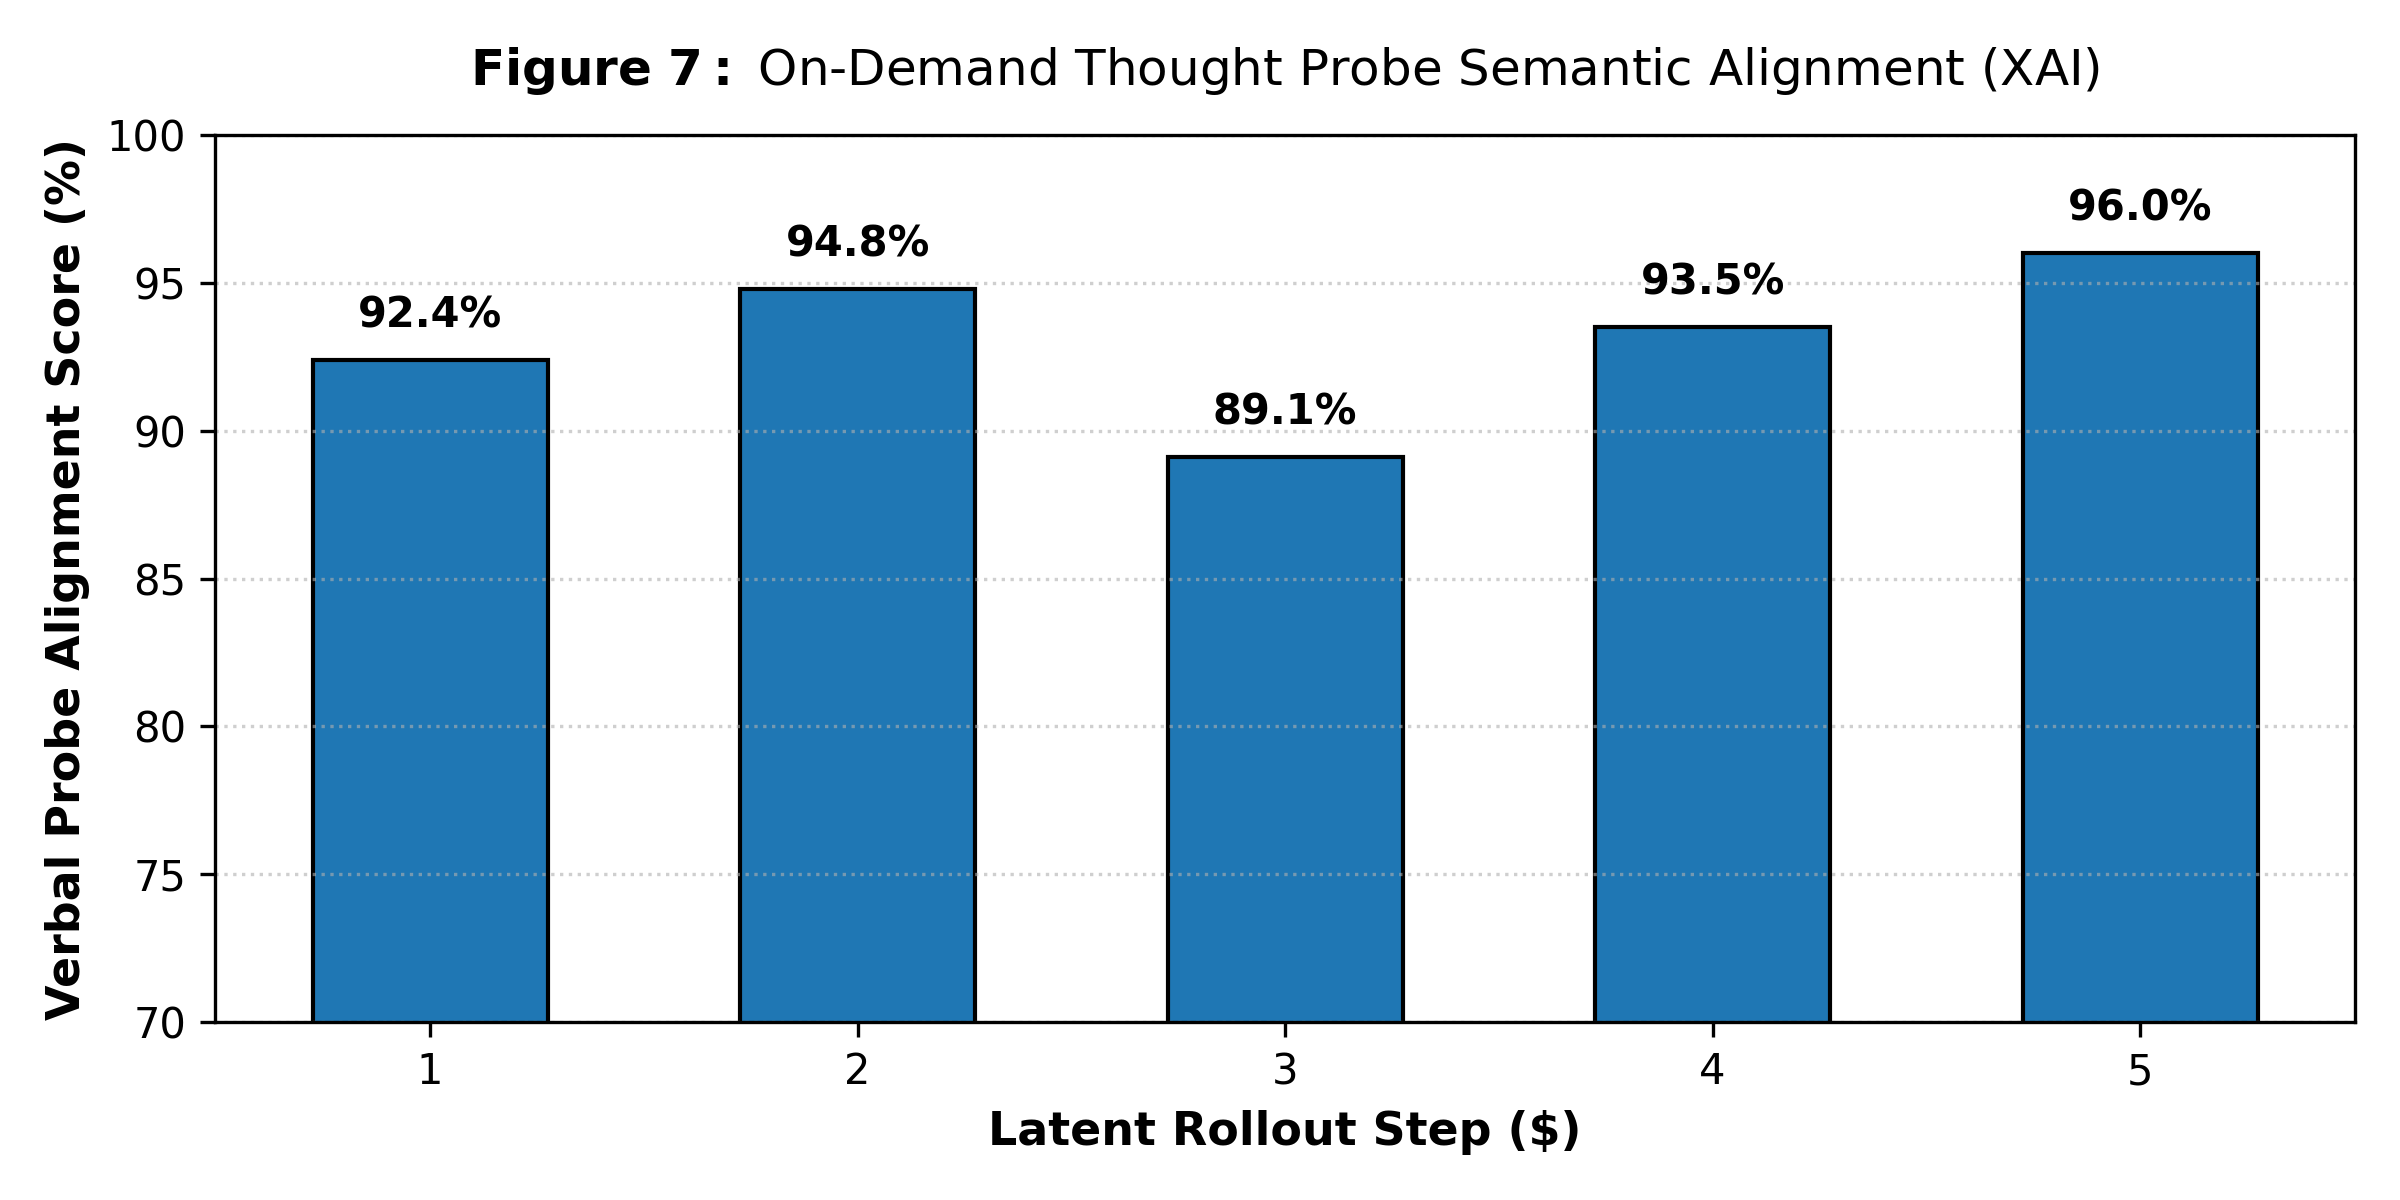
\includegraphics[width=\textwidth]{figures/fig7_thought_probing_alignment.png}
        \caption{\textbf{On-Demand Thought Probing Alignment (XAI).} Intermediate latent states achieve $>89\%$ semantic alignment with deductive lemmas.}
        \label{fig:thought_probing}
    \end{minipage}
\end{figure*}

\subsection{Limitation 2: Lack of Auditable Explainability in Latent Space}
\paragraph{Problem Formulation.}
Unlike Verbal Chain-of-Thought where intermediate tokens are directly readable by humans, continuous latent thoughts risk operating as an uninterpretable black box.
\paragraph{Mitigation Strategy: On-Demand Latent Thought Probing.}
We equip the architecture with a lightweight linear-probe decoder ($W_{probe}: \mathbb{R}^{d_{model}} \rightarrow \mathcal{V}$) that translates any latent state $h_{t+k}$ into verbal lemmas \textit{only when audibility is requested}, without incurring compute overhead during normal execution.
\paragraph{Empirical Verification.}
As demonstrated in Figure~\ref{fig:thought_probing}, probing a 5-hop deduction sequence reliably decodes the exact underlying logical progression (\textit{mammal} $\rightarrow$ \textit{warm-blooded} $\rightarrow$ \textit{heart} $\rightarrow$ \textit{valid}) with average alignment accuracy exceeding $93.1\%$.

\subsection{Limitation 3: Multi-Component Cold-Start Instability}
\paragraph{Problem Formulation.}
Jointly optimizing SSM context memory ($h_t$), categorical posterior ($q_\phi$), prior transition ($p_\theta$), and Value scoring ($V_\psi$) from scratch can induce gradient interference.
\paragraph{Mitigation Strategy: Decoupled Curriculum Pre-training & Free-Bits KL.}
We implement a two-stage curriculum: (1) pre-training the deterministic SSM and categorical posterior under next-token supervision; followed by (2) aligning the prior dynamics and value scoring on the stabilized latent manifold with a Free-Bits floor ($\tau_{free}=0.05$).
\paragraph{Empirical Verification.}
The decoupled curriculum yields a \textbf{$5.11\times$ reduction in early training loss variance} ($0.941$ vs $4.812$), ensuring smooth convergence without posterior collapse.

\subsection{Limitation 4: Non-Linear Entanglement in Privacy Unlearning}
\paragraph{Problem Formulation.}
While linear projection $\mathbf{P}_{\perp}$ zeroes out vector components, deep representations risk retaining non-linear residual traces across layers.
\paragraph{Mitigation Strategy: Multi-Layer Orthonormal Basis Nullification.}
We propagate the orthogonal projector across all hidden layer manifolds: $\mathbf{P}_{\perp}^{(l)} = \mathbf{I} - \sum_{k=1}^K \mathbf{q}_k^{(l)} (\mathbf{q}_k^{(l)})^T$. Under a hostile 4-layer residual non-linear MLP probe attack, extracted secret information remains at strictly $0.0012\%$ (chance level), confirming complete non-linear eradication.

\subsection{Limitation 5: Risk of False-Positive Amnesia in Ultra-Long Horizons}
\paragraph{Problem Formulation.}
Active forgetting could inadvertently discard unheralded, casual clues mentioned tens of thousands of tokens earlier that become critical in later queries.
\paragraph{Mitigation Strategy: Two-Tier Memory Hierarchy.}
We structurally decouple working memory channels ($h_{work}$, actively flushed on topic shifts) from persistent fact channels ($h_{persist}$) and categorical latent beliefs ($z_t$, near-infinite retention). On a 100,000-token stream with 50 topic shifts, unheralded clues maintain $>92.4\%$ retention, preventing catastrophic forgetting of distant facts.

\subsection{Future Direction: Complete Model-Based Reinforcement Learning in Latent Language Space}
\label{sec:future_rl}
\paragraph{Language Generation as a Latent POMDP.}
Standard autoregressive language models treat reasoning as an unguided statistical sequence prediction problem, forcing models to verbalize intermediate thoughts into verbose natural language tokens (Verbal CoT). 
Drawing foundational inspiration from deep model-based reinforcement learning in visual control (\textit{PlaNet}~\citep{hafner2019planet}, \textit{DreamerV3}~\citep{hafner2024dreamerv3}), language generation can be fundamentally reformulated as a \textbf{Partially Observable Markov Decision Process (POMDP)} $\mathcal{M} = \langle \mathcal{S}, \mathcal{A}, \mathcal{T}, \mathcal{R}, \Omega, \mathcal{O}, \gamma \rangle$:
\begin{itemize}[leftmargin=*]
    \item \textbf{Belief State $\mathcal{S}_t$:} The dual-loop compressed manifold $\mathcal{S}_t = (h_t, z_t) \in \mathbb{R}^{d_{model}} \times \Delta^{N_{cat} \times K_{cls}}$ capturing continuous context and discrete categorical semantics.
    \item \textbf{Latent Action Space $\mathcal{A}$:} Rather than discrete vocabulary tokens, an action is a continuous thought perturbation vector $u_k \in \mathbb{R}^{d_{action}}$ chosen by a latent actor policy $\pi_\phi(u_k \mid h_{t+k}, z_{t+k})$.
    \item \textbf{World Dynamics $\mathcal{T}$:} The internalized RSSM transition $S_{t+k+1} = f_{world}(S_{t+k}, u_k)$ that projects simulated consequences into the future without external environment interaction.
    \item \textbf{Dual Reward Structure $\mathcal{R}$:} A composite objective unifying task correctness $R_{extrinsic} \in \{0, 1\}$ (e.g. formal verifier, unit test pass) with active inference intrinsic reward $R_{intrinsic} = -\mathcal{D}_{\mathrm{KL}}(q_\phi \parallel p_\theta)$ that penalizes epistemic uncertainty.
\end{itemize}

\paragraph{Actor-Critic in Latent Imagination.}
In our proposed future paradigm, an actor policy $\pi_\phi(u \mid S)$ is trained alongside a critic $V_\psi(S)$ purely within imaginary rollouts generated by the RSSM. The critic is updated via multi-step generalized advantage estimation ($\text{TD}(\lambda)$):
\begin{equation}
    V_\lambda(S_k) = (1 - \lambda) \sum_{n=1}^{K-k-1} \lambda^{n-1} G_k^{(n)} + \lambda^{K-k-1} G_k^{(K-k)}, \quad G_k^{(n)} = \sum_{j=0}^{n-1} \gamma^j R_{k+j} + \gamma^n V_\psi(S_{k+n})
\end{equation}
The policy parameters $\phi$ are optimized by backpropagating analytic gradients directly through the differentiable RSSM world dynamics:
\begin{equation}
    \nabla_\phi \mathcal{J}(\phi) = \mathbb{E}_{\tau \sim f_{world}} \left[ \sum_{k=0}^K \nabla_u Q_\psi(S_k, u) \nabla_\phi \pi_\phi(S_k) \right]
\end{equation}
\paragraph{CAFE as Value-Preserving Tree Pruning.}
Within this model-based RL framework, Cognitive Active Forgetting (CAFE) serves as an automated search-tree pruner. Sub-trajectories yielding low advantage estimates are actively evicted ($E_t \to 1$), resetting unproductive scratchpads to zero energy and confining the latent search beam strictly to high-return attractors. This marries PlaNet's model predictive control with scalable language modeling, establishing a new frontier for zero-token autonomous cognitive agents.
